\documentclass[a4paper,11pt]{extarticle}
\usepackage[utf8]{inputenc}
\usepackage[T1]{fontenc}
\usepackage{graphicx}
\usepackage{xcolor}
\usepackage{tikz}

\usepackage{amsmath,amssymb,textcomp}
\everymath{\displaystyle}

\usepackage{times}
\renewcommand\familydefault{\sfdefault}
\usepackage{tgheros}
\usepackage[defaultmono,scale=0.85]{droidmono}

\usepackage{multicol}
\setlength{\columnseprule}{0pt}
\setlength{\columnsep}{20.0pt}


\usepackage{geometry}
\geometry{
a4paper,
total={210mm,297mm},
left=10mm,right=10mm,top=10mm,bottom=15mm}

\linespread{1.3}


% custom title
\makeatletter
\renewcommand*{\maketitle}{%
\noindent
\begin{minipage}{0.4\textwidth}

\begin{tikzpicture}
\node[rectangle,rounded corners=6pt,inner sep=10pt,fill=blue!50!black,text width= 0.95\textwidth] {\color{white}\Huge \@title};
\end{tikzpicture}
\end{minipage}
\hfill
\begin{minipage}{0.55\textwidth}
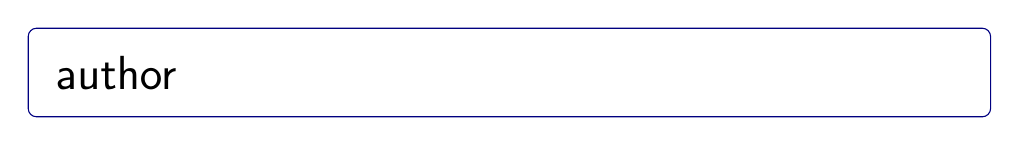
\begin{tikzpicture}
\node[rectangle,rounded corners=3pt,inner sep=10pt,draw=blue!50!black,text width= 0.95\textwidth] {\LARGE \@author};
\end{tikzpicture}
\end{minipage}
\bigskip\bigskip
}%
\makeatother

% custom section
\usepackage[explicit]{titlesec}
\newcommand*\sectionlabel{}
\titleformat{\section}
  {\gdef\sectionlabel{}
   \normalfont\sffamily\Large\bfseries\scshape}
  {\gdef\sectionlabel{\thesection\ }}{0pt}
  {
\noindent
\begin{tikzpicture}
\node[rectangle,rounded corners=3pt,inner sep=4pt,fill=blue!50!black,text width= 0.95\columnwidth] {\color{white}\sectionlabel#1};
\end{tikzpicture}
  }
\titlespacing*{\section}{0pt}{15pt}{10pt}


% custom footer
\usepackage{fancyhdr}
\makeatletter
\pagestyle{fancy}
\fancyhead{}
\fancyfoot[C]{\footnotesize \textcopyright\ \@date\ \ \@author}
\renewcommand{\headrulewidth}{0pt}
\renewcommand{\footrulewidth}{0pt}
\makeatother


\title{QFT}
\author{Rodrigo Souza}
\date{2016}



\begin{document}

\maketitle

\begin{multicols*}{2}


\section{Componentes covariantes}


\begin{eqnarray*}
\partial_{\mu}& = & \frac{\partial}{\partial x^{\mu}} = \left(\frac{\partial}{\partial t}, \frac{\partial}{\partial x^{i}} \right)^T = \left(\frac{\partial}{\partial t}, \frac{\partial}{\partial X_{i}} \right)^T\\
\partial^{\mu}& = & \frac{\partial}{\partial x_{\mu}} = \left(\frac{\partial}{\partial t}, \frac{\partial}{\partial x_{i}} \right)^T = \left(\frac{\partial}{\partial t}, - \frac{\partial}{\partial X_{i}} \right)^T\\
\end{eqnarray*}


\section{Equações de Euler-Lagrange}


\begin{equation*}
\frac{\partial }{\partial x^{\mu}} \left( \frac{\mathcal{L}}{\partial \phi^{r}_{,\mu}}\right) - \frac{\mathcal{L}}{\partial \phi^{r}} = 0
\end{equation*}

\begin{equation*}
\pi_r = \frac{\partial \mathcal{L}}{\partial \dot{\phi}^r}
\end{equation*}


\begin{equation*}
\mathcal{H} = \pi_r \dot{\phi}^r - \mathcal{L}
\end{equation*}

\section{Klein-Gordon}


\begin{equation*}
\mathcal{L}_{0}^{0} = \partial_{\alpha}\phi^{\dagger}\partial^{\alpha}\phi - \mu \phi^{\dagger} \phi
\end{equation*}


\end{multicols*}

\end{document}
